\documentclass[hyperref=colorlinks]{beamer}
\mode<presentation>
\usetheme{iclpt}
\setbeamertemplate{navigation symbols}{}
\setbeamertemplate{headline}{
\begin{beamercolorbox}[leftskip=.2cm,rightskip=.2cm,topskip=.2cm,ht=1.1cm,dp=0.1cm,wd=\textwidth]{institute in head/foot}
  
\includegraphics[height=1cm]{icl.pdf}
  \hfill
  
\includegraphics[height=1cm]{../Pics/CMS-Color.pdf}
\end{beamercolorbox}
}
\setbeamertemplate{footline}{
\begin{beamercolorbox}[ht=.55cm,dp=0.4cm,wd=\textwidth,leftskip=.3cm]{author in head/foot}%
  \begin{minipage}[c]{5cm}%
    \usebeamerfont{author in head/foot}
    \insertshortauthor 
    \insertshorttitle
    \end{minipage}\hfill%
  \insertframenumber{} / \pageref{lastframe}
  \hfill
  \begin{minipage}{6cm}
    \hfill
  \end{minipage}
\end{beamercolorbox}%
}

\usepackage{color}
\usepackage{tabularx,colortbl}
\usepackage{graphicx}
\usepackage{pdfpages}
\usepackage{feynmp}
\DeclareGraphicsRule{*}{mps}{*}{}

\title{\vspace{-0.2cm} VBF Higgs to Invisible}
\subtitle{HIG-14-038, AN-14-243\vspace{-0.7cm}}
\author[]{}%\underline{P. Dunne}} % A.M. Magnan and A. Nikitenko Joao Pela with \\ R. Aggleton, J. Brooke: Bristol \\ C.Asawangtrakuldee, Q.Li: Peking \\ P. Srimanobhas: Chulalongkorn \\ S. Kumar, K. Mazumdar: Mumbai}
\titlegraphic{
  \vspace{-0.7cm}
  %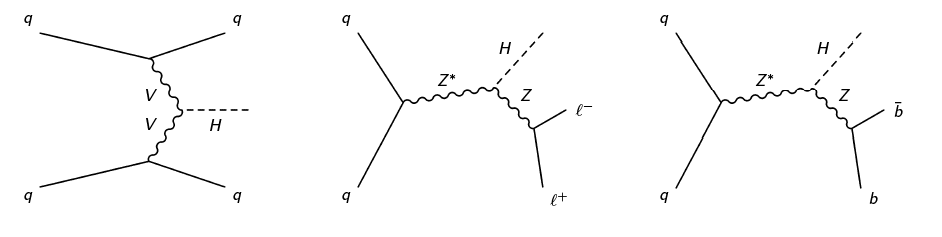
\includegraphics[width=\textwidth]{TalkPics/invcomb021213/feyndiags}
  %% \begin{fmfgraph*}(100,70)
  %%         \fmfleft{i1,i2}
  %%         \fmfright{o1,o2,o3}
  %%         \fmf{fermion}{i1,v1,o1}
  %%         \fmf{fermion}{i2,v2,o3}
  %%         \fmf{phantom,tension=4/5}{v1,v2}
  %%         \fmffreeze
  %%         \fmf{photon,label=$W,,Z$}{v1,v3}
  %%         \fmf{photon,label=$W,,Z$}{v2,v3}
  %%         \fmf{dashes}{v3,o2}
  %%         \fmflabel{$q$}{i1}
  %%         \fmflabel{$q$}{i2}
  %%         \fmflabel{$q$}{o1}
  %%         \fmflabel{$q$}{o3}
  %%         \fmflabel{$H$}{o2}
  %%       \end{fmfgraph*}
}
\date{}
\begin{document}
\begin{fmffile}{higgsexoupdatefeyndiags}

%TITLE PAGE
\section{Title}
\begin{frame}
  \titlepage
  
\end{frame}

\begin{frame}
  \frametitle{Overview}
  \begin{block}{}
    \begin{itemize}
    \item Investigate whether ATLAS/CMS difference is due to use of $Z\rightarrow\mu\mu$ sample
    \item[-] They use a real $Z\rightarrow\nu\nu$ sample
    \item Our $Z\rightarrow\nu\nu$ sample is missing the $H_{T}<50$ GeV region
    \end{itemize}
    \end{block}
\end{frame}

\begin{frame}
  \frametitle{HT makeup of $Z\rightarrow\nu\nu$ sample}
  \begin{columns}
    \column{.5\textwidth}
  \begin{block}{}
    \scriptsize
    \begin{itemize}
    \item Signal region selection applied
    \item No steps visible due to $H_{T}$ binning
    \item $Z\rightarrow\nu\nu$ appears slightly softer than $Z\rightarrow\mu\mu$
    \item $H_{T}>50$ GeV cut doesn't seem to bias the sample in this region
    \end{itemize}
  \end{block}
  \column{.6\textwidth}
  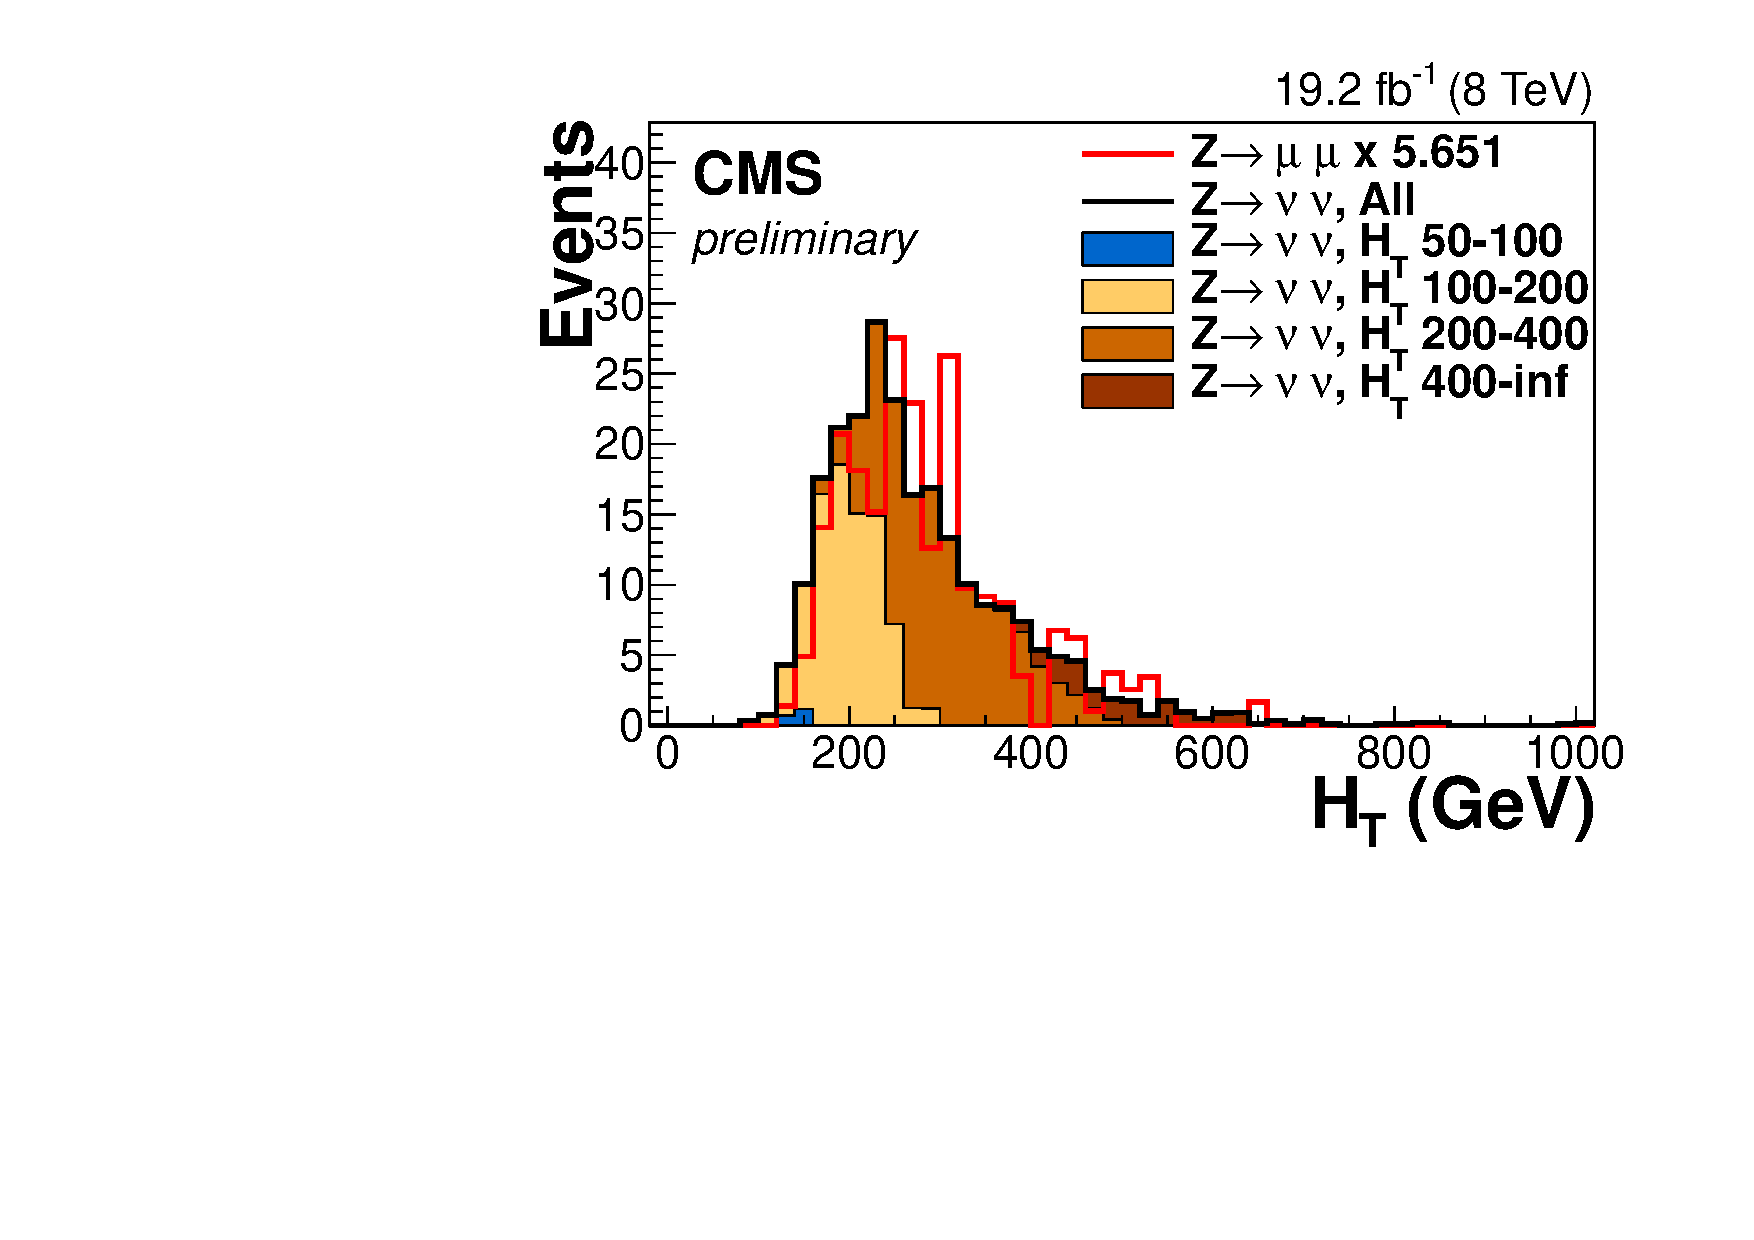
\includegraphics[width=\textwidth]{TalkPics/znunumcstudy200415/htdist.pdf}
  \end{columns}
\end{frame}

%!!MENTION RELATIVE YIELDS
%!!MENTION NUNU A BIT SOFTER
%!!MENTION UNCLUSTERED ISSUE

\begin{frame}
  \frametitle{Distribution comparison}
  \begin{block}{}
    \scriptsize
    \begin{itemize}
    \item Normalise $Z\rightarrow\nu\nu$ and $Z\rightarrow\mu\mu$ to 1 and compare
    \end{itemize}
  \end{block}
      
      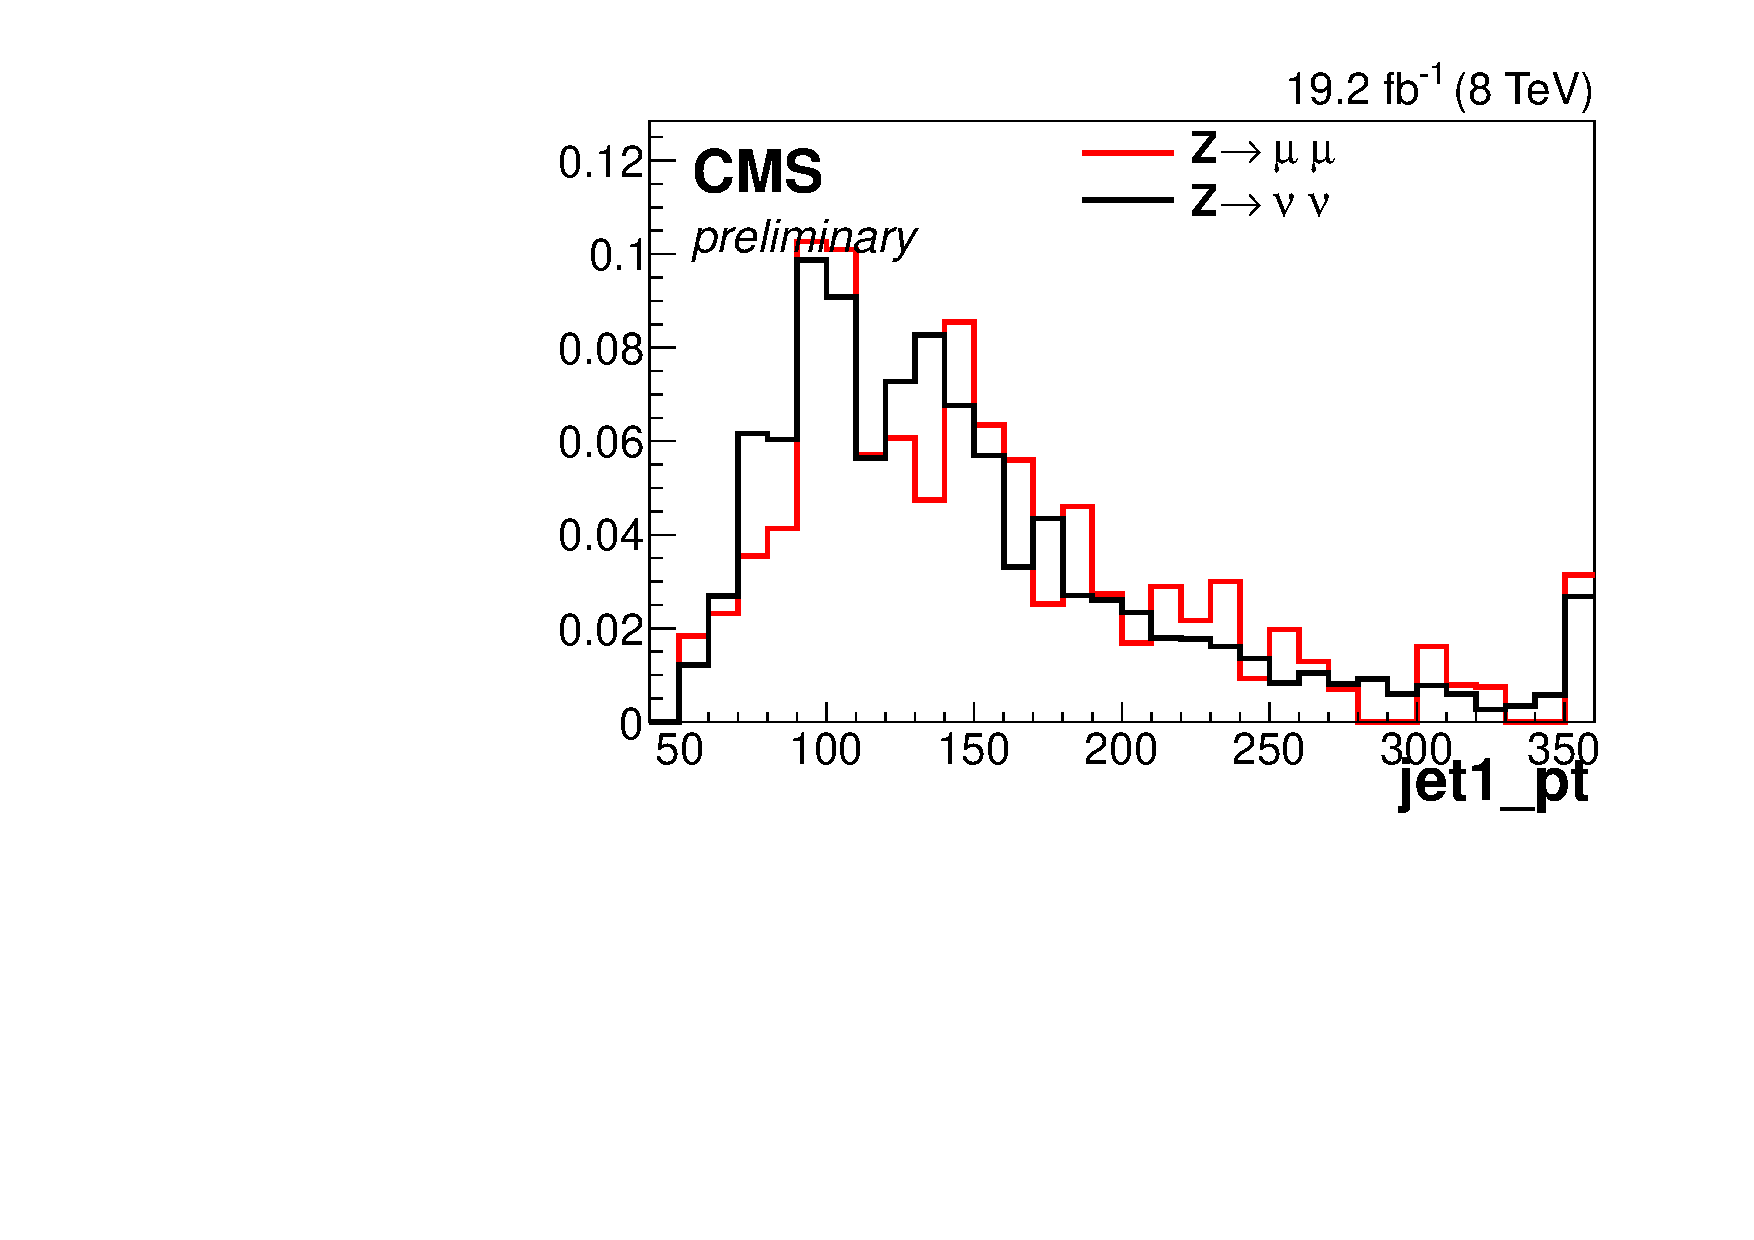
\includegraphics[width=.5\textwidth]{TalkPics/znunumcstudy200415/znunustudy_jet1_pt.pdf}
      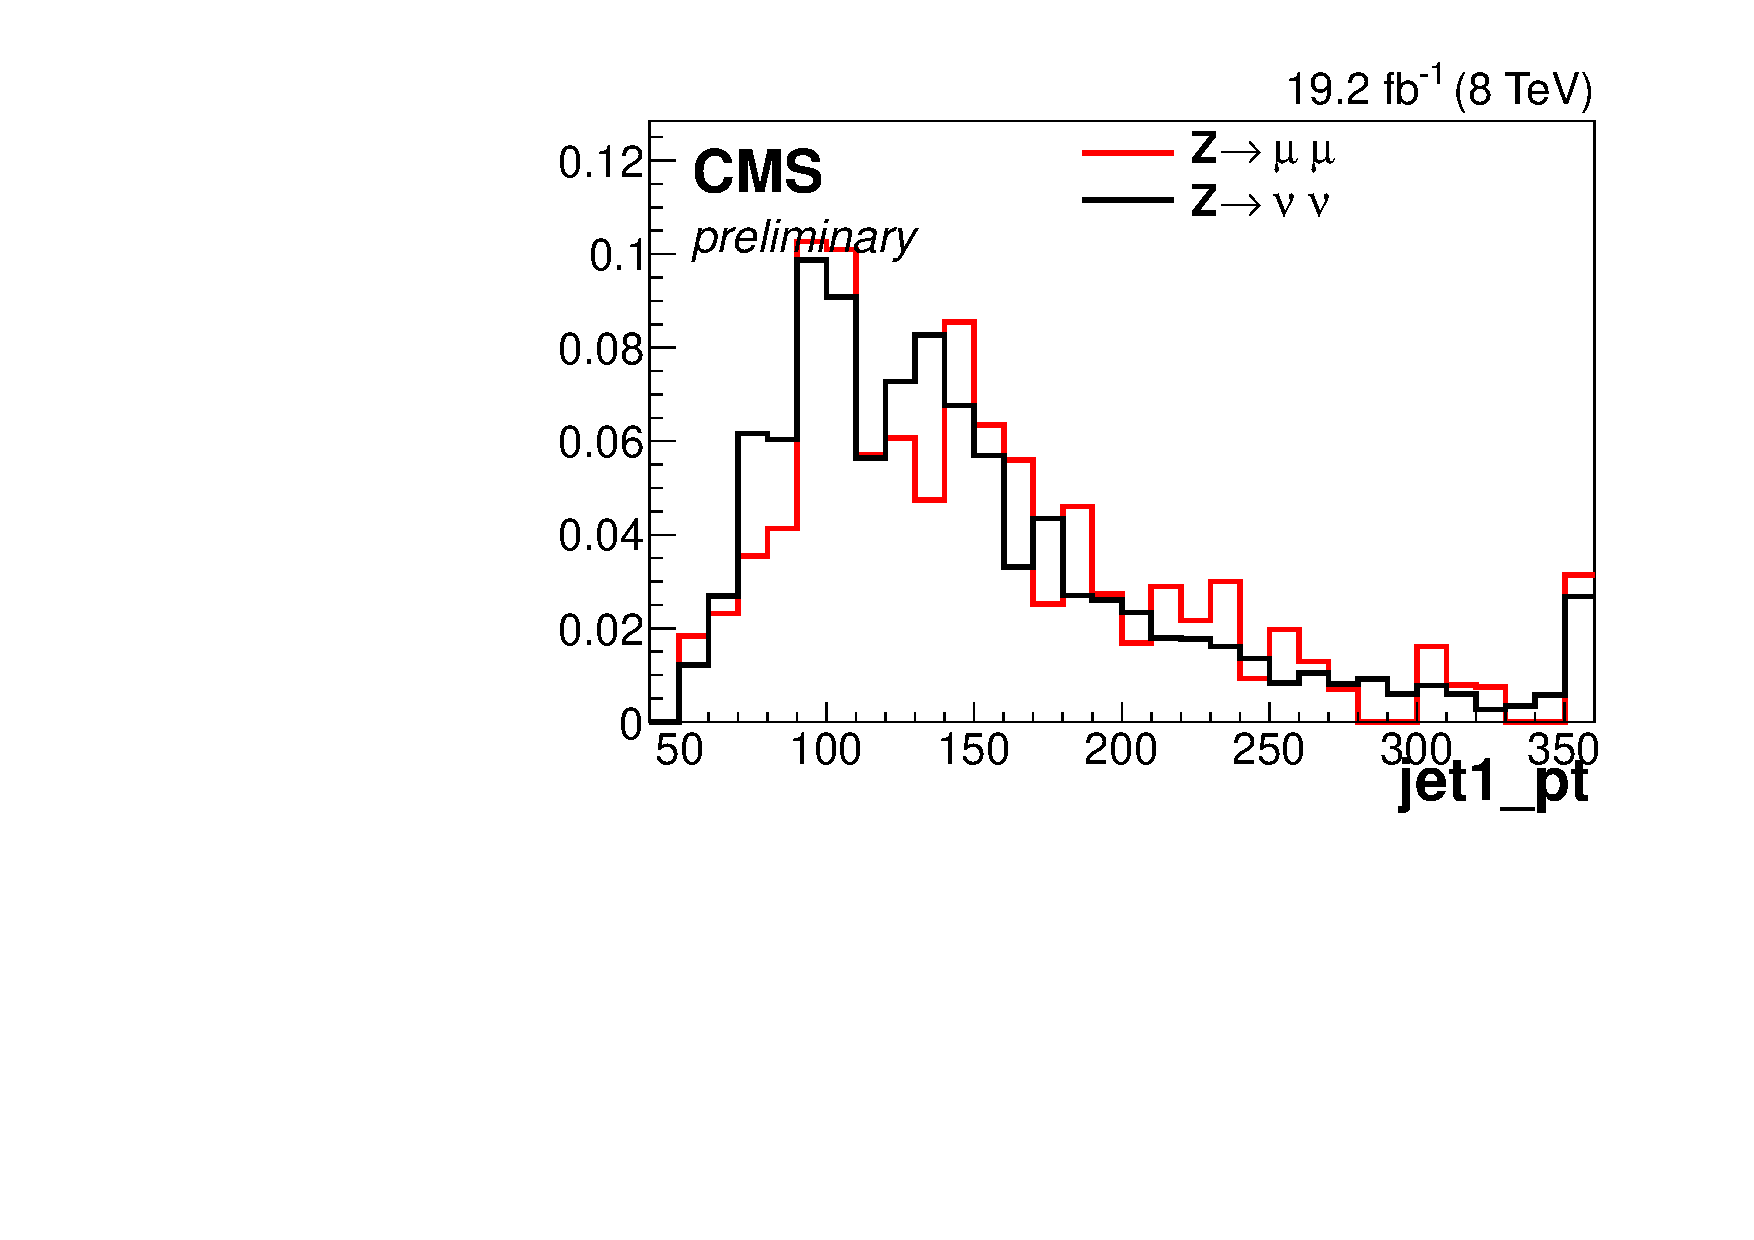
\includegraphics[width=.5\textwidth]{TalkPics/znunumcstudy200415/znunustudy_jet1_pt.pdf}

\end{frame}

\begin{frame}
  \frametitle{Distribution comparison}
  \begin{block}{}
    \scriptsize
    \begin{itemize}
    \item Normalise $Z\rightarrow\nu\nu$ and $Z\rightarrow\mu\mu$ to 1 and compare
    \end{itemize}
  \end{block}
      
      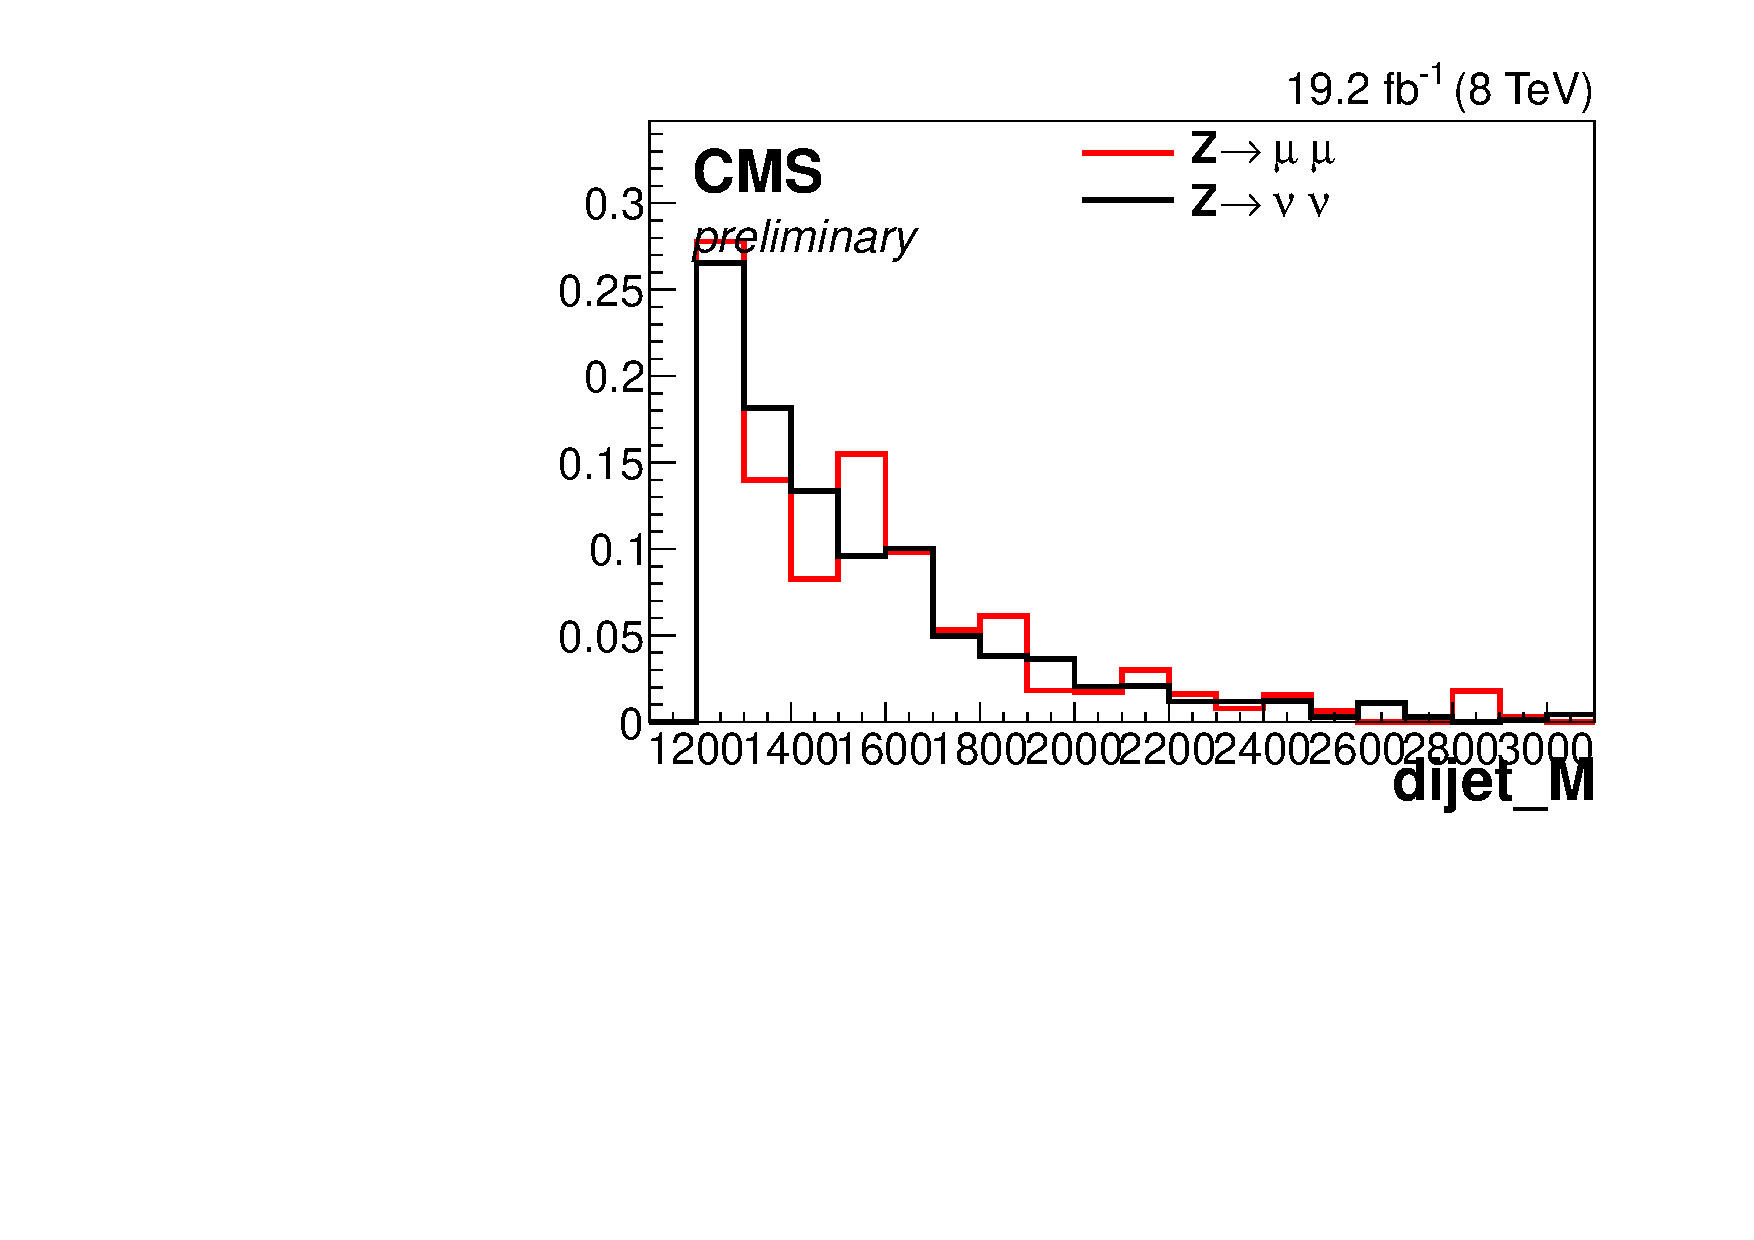
\includegraphics[width=.5\textwidth]{TalkPics/znunumcstudy200415/znunustudy_dijet_M.pdf}
      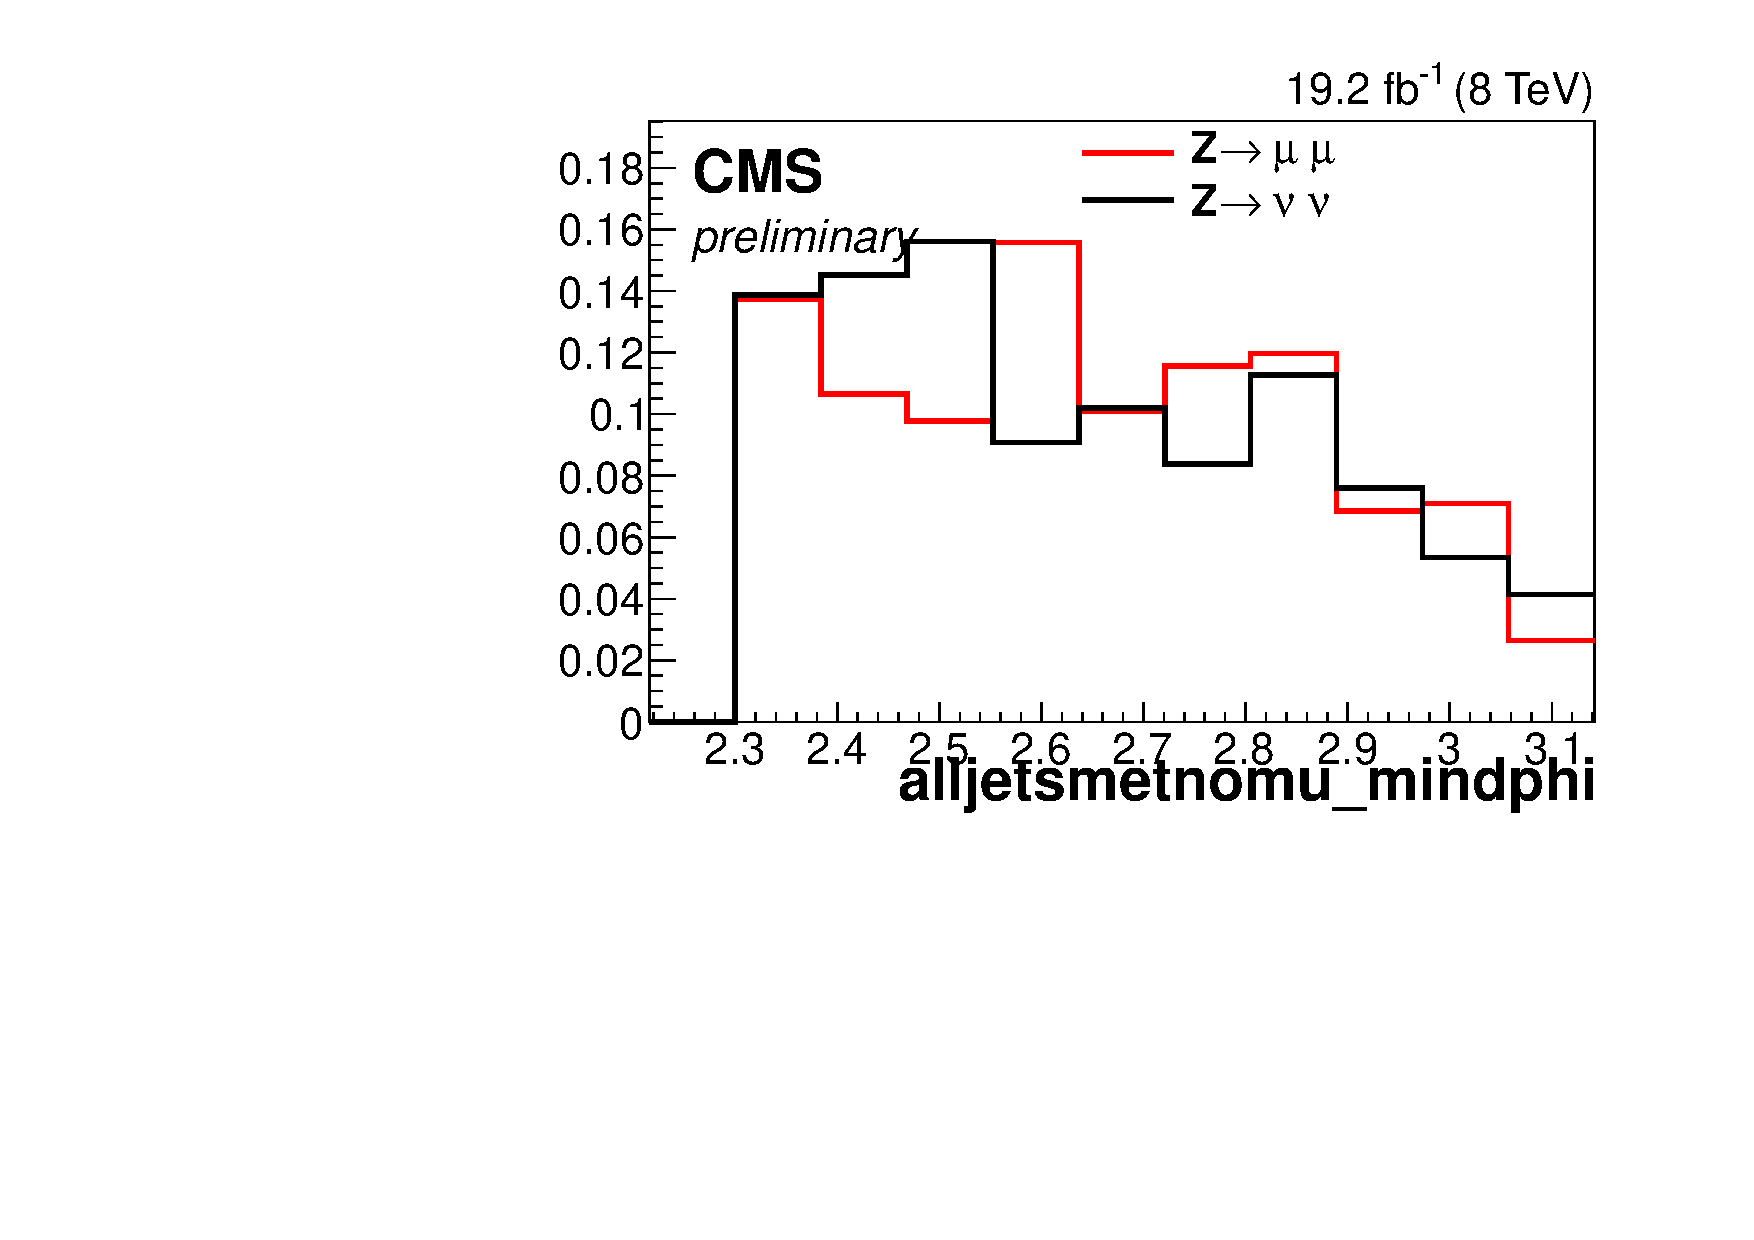
\includegraphics[width=.5\textwidth]{TalkPics/znunumcstudy200415/znunustudy_alljetsmetnomu_mindphi.pdf}

\end{frame}

\begin{frame}
  \frametitle{Distribution comparison}
  \begin{block}{}
    \scriptsize
    \begin{itemize}
    \item Normalise $Z\rightarrow\nu\nu$ and $Z\rightarrow\mu\mu$ to 1 and compare
    \end{itemize}
  \end{block}
      
      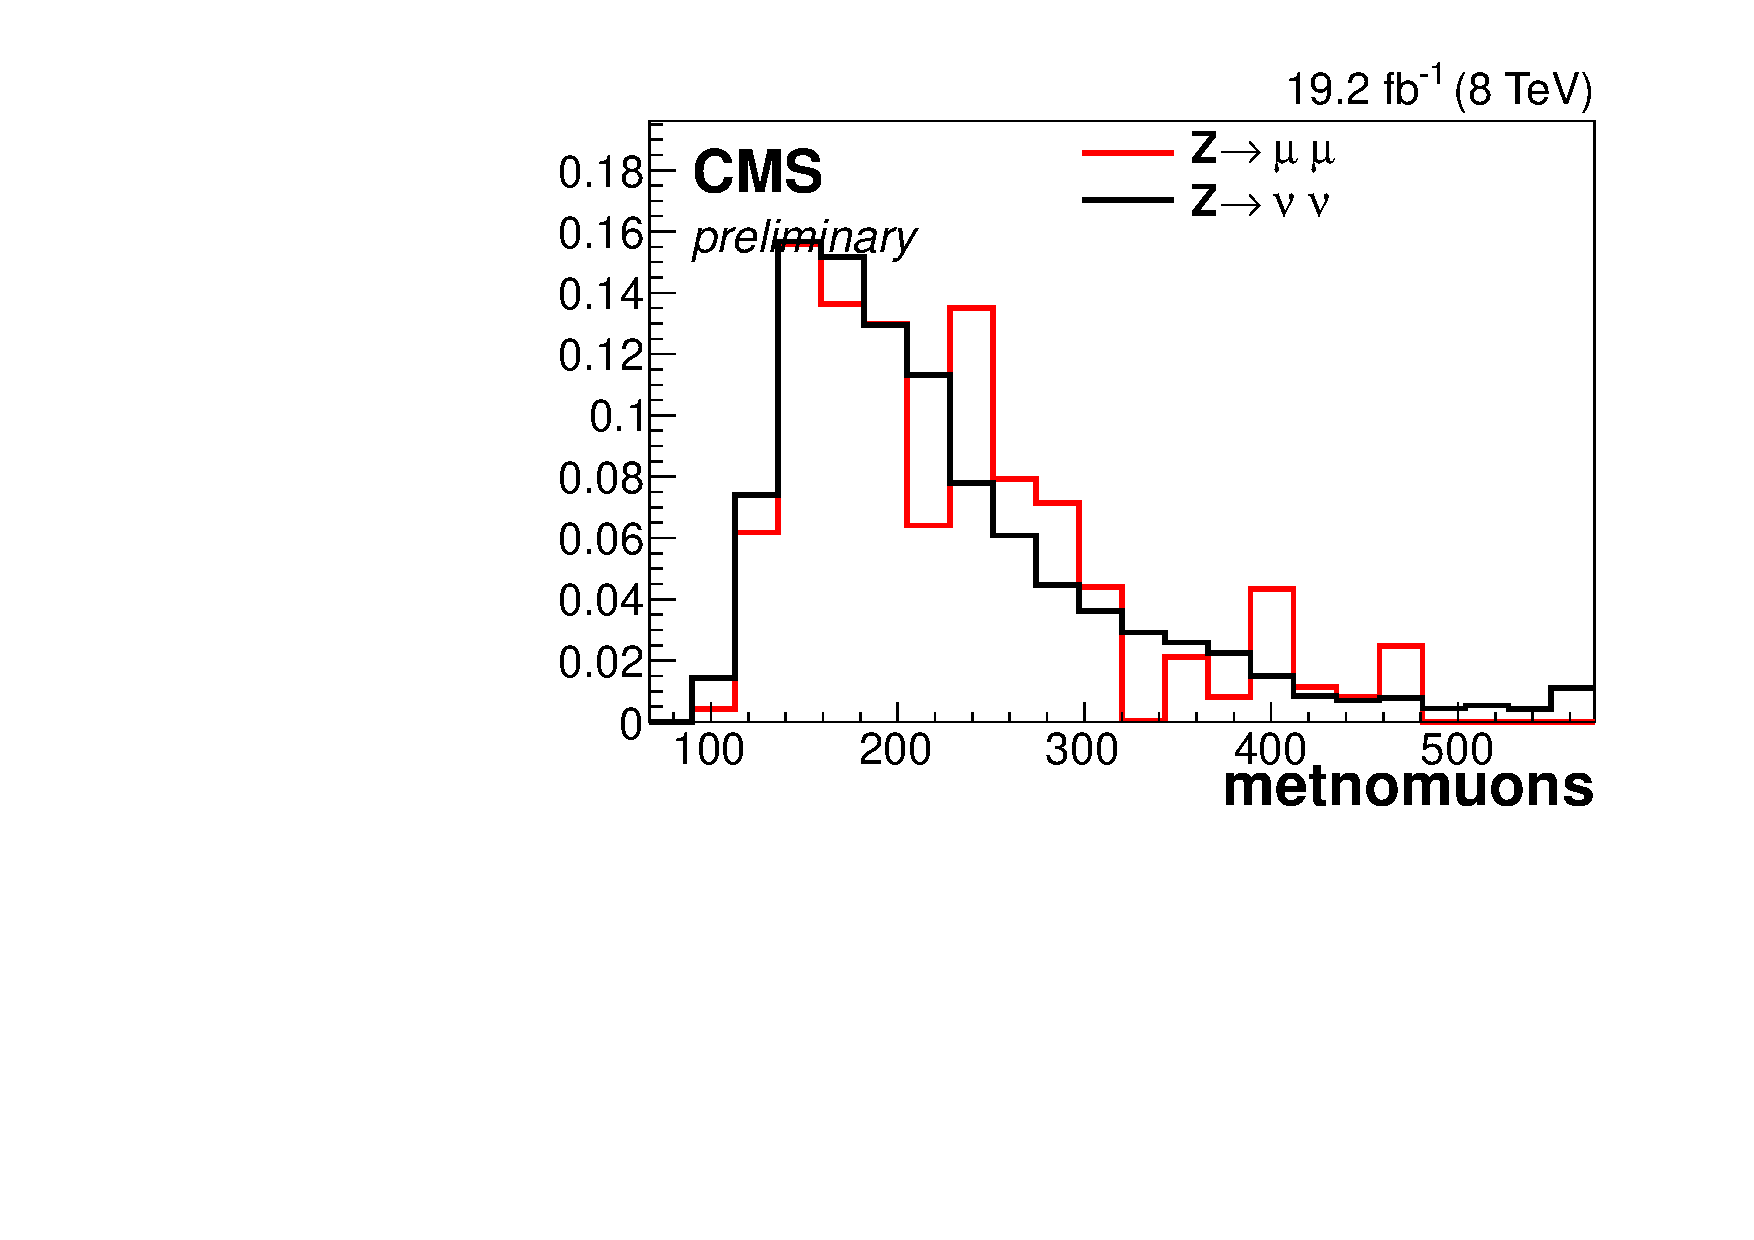
\includegraphics[width=.5\textwidth]{TalkPics/znunumcstudy200415/znunustudy_metnomuons.pdf}
      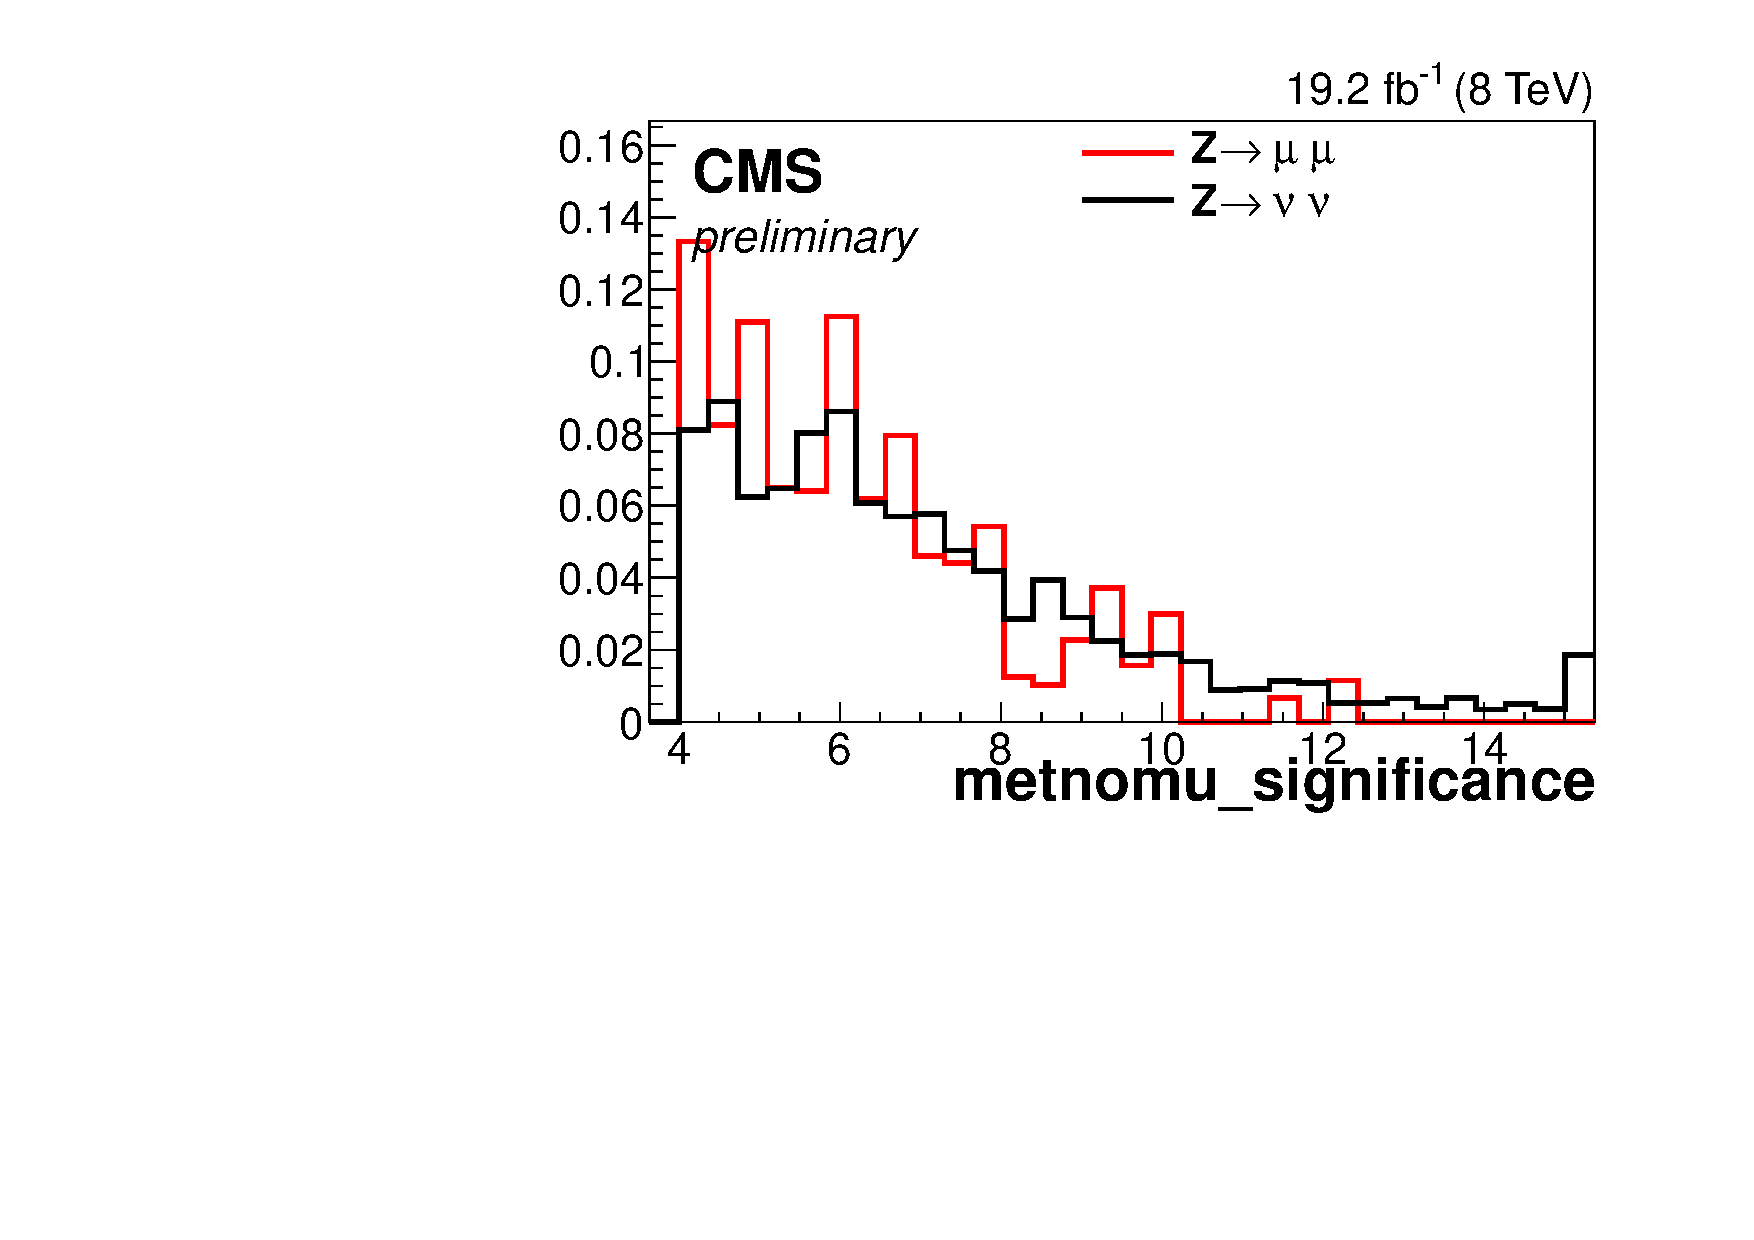
\includegraphics[width=.5\textwidth]{TalkPics/znunumcstudy200415/znunustudy_metnomu_significance.pdf}

\end{frame}

\begin{frame}
  \frametitle{Distribution comparison}
  \begin{block}{}
    \scriptsize
    \begin{itemize}
    \item Normalise $Z\rightarrow\nu\nu$ and $Z\rightarrow\mu\mu$ to 1 and compare
    \end{itemize}
  \end{block}
      
  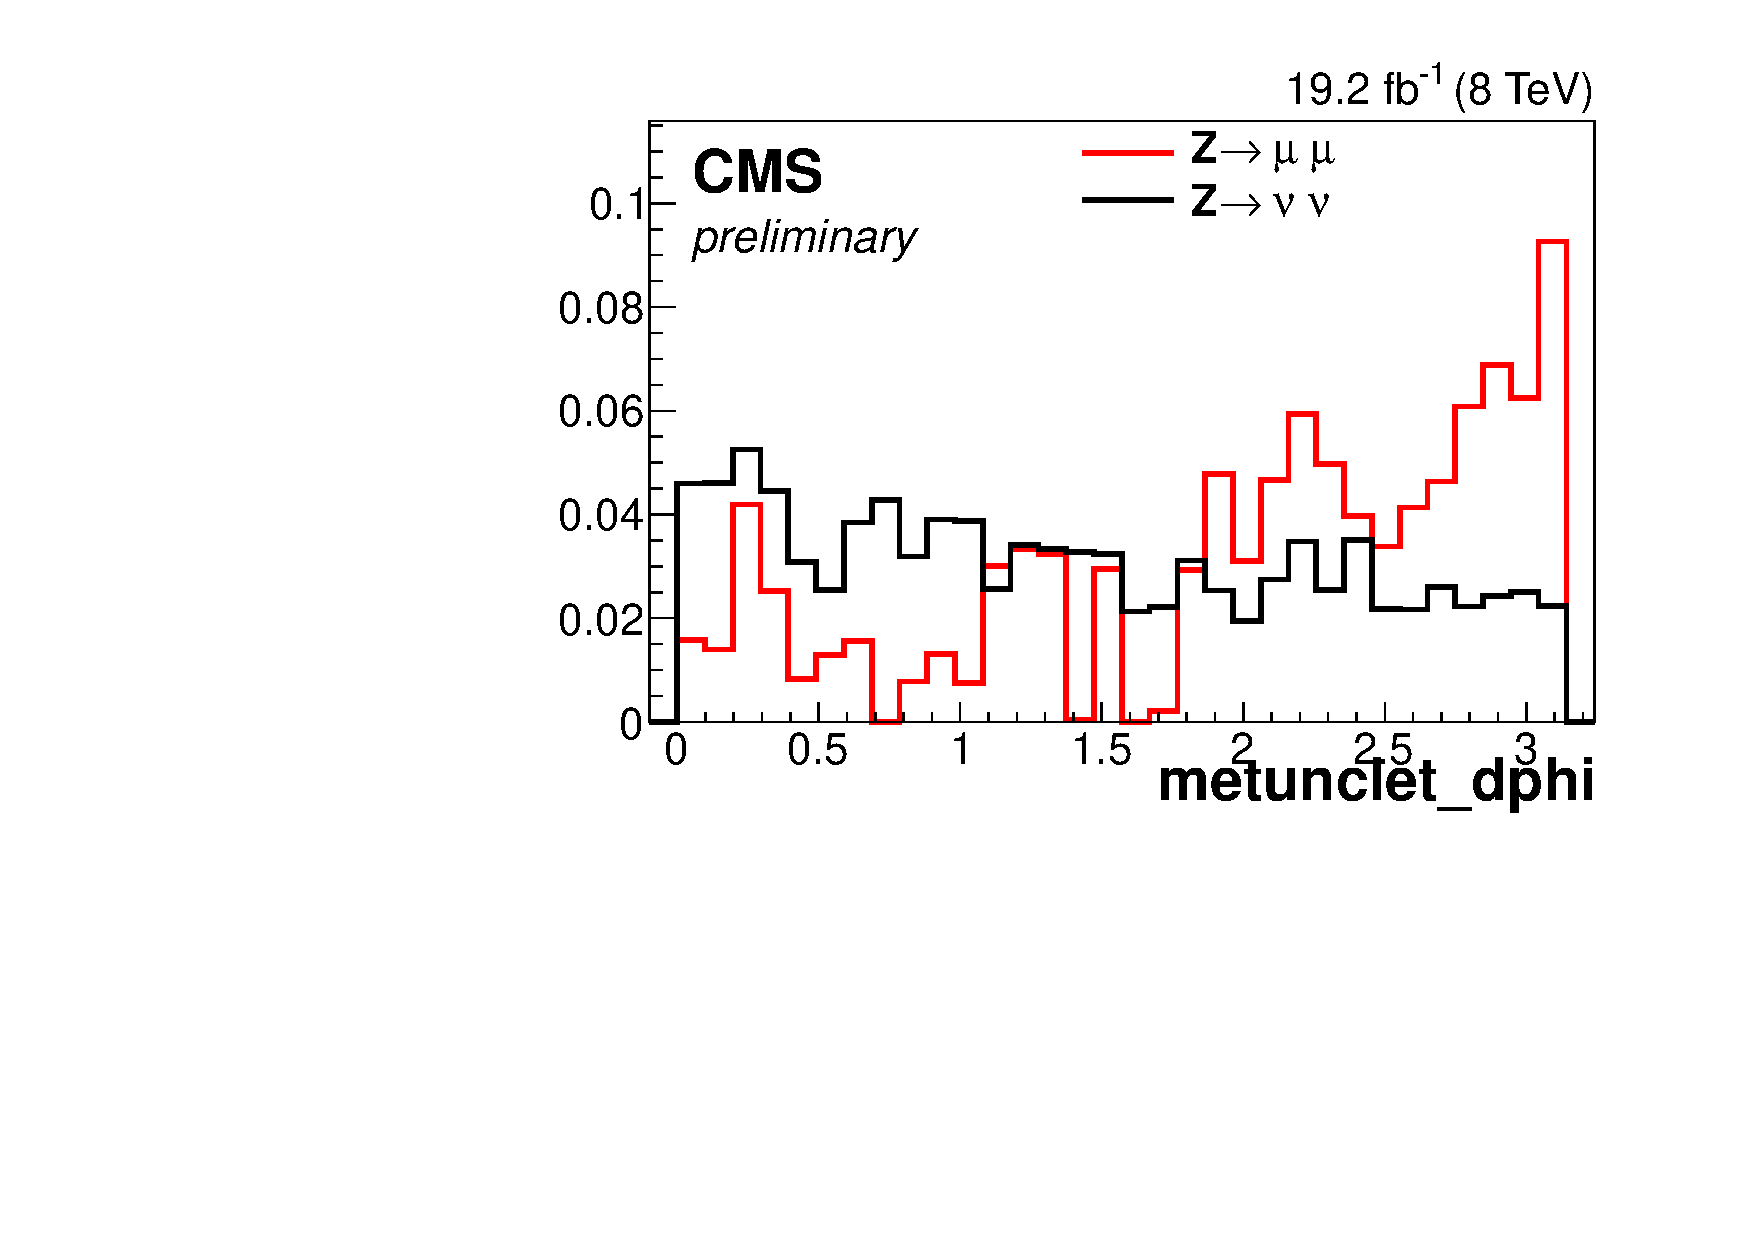
\includegraphics[width=.5\textwidth]{TalkPics/znunumcstudy200415/znunustudy_metunclet_dphi.pdf}
  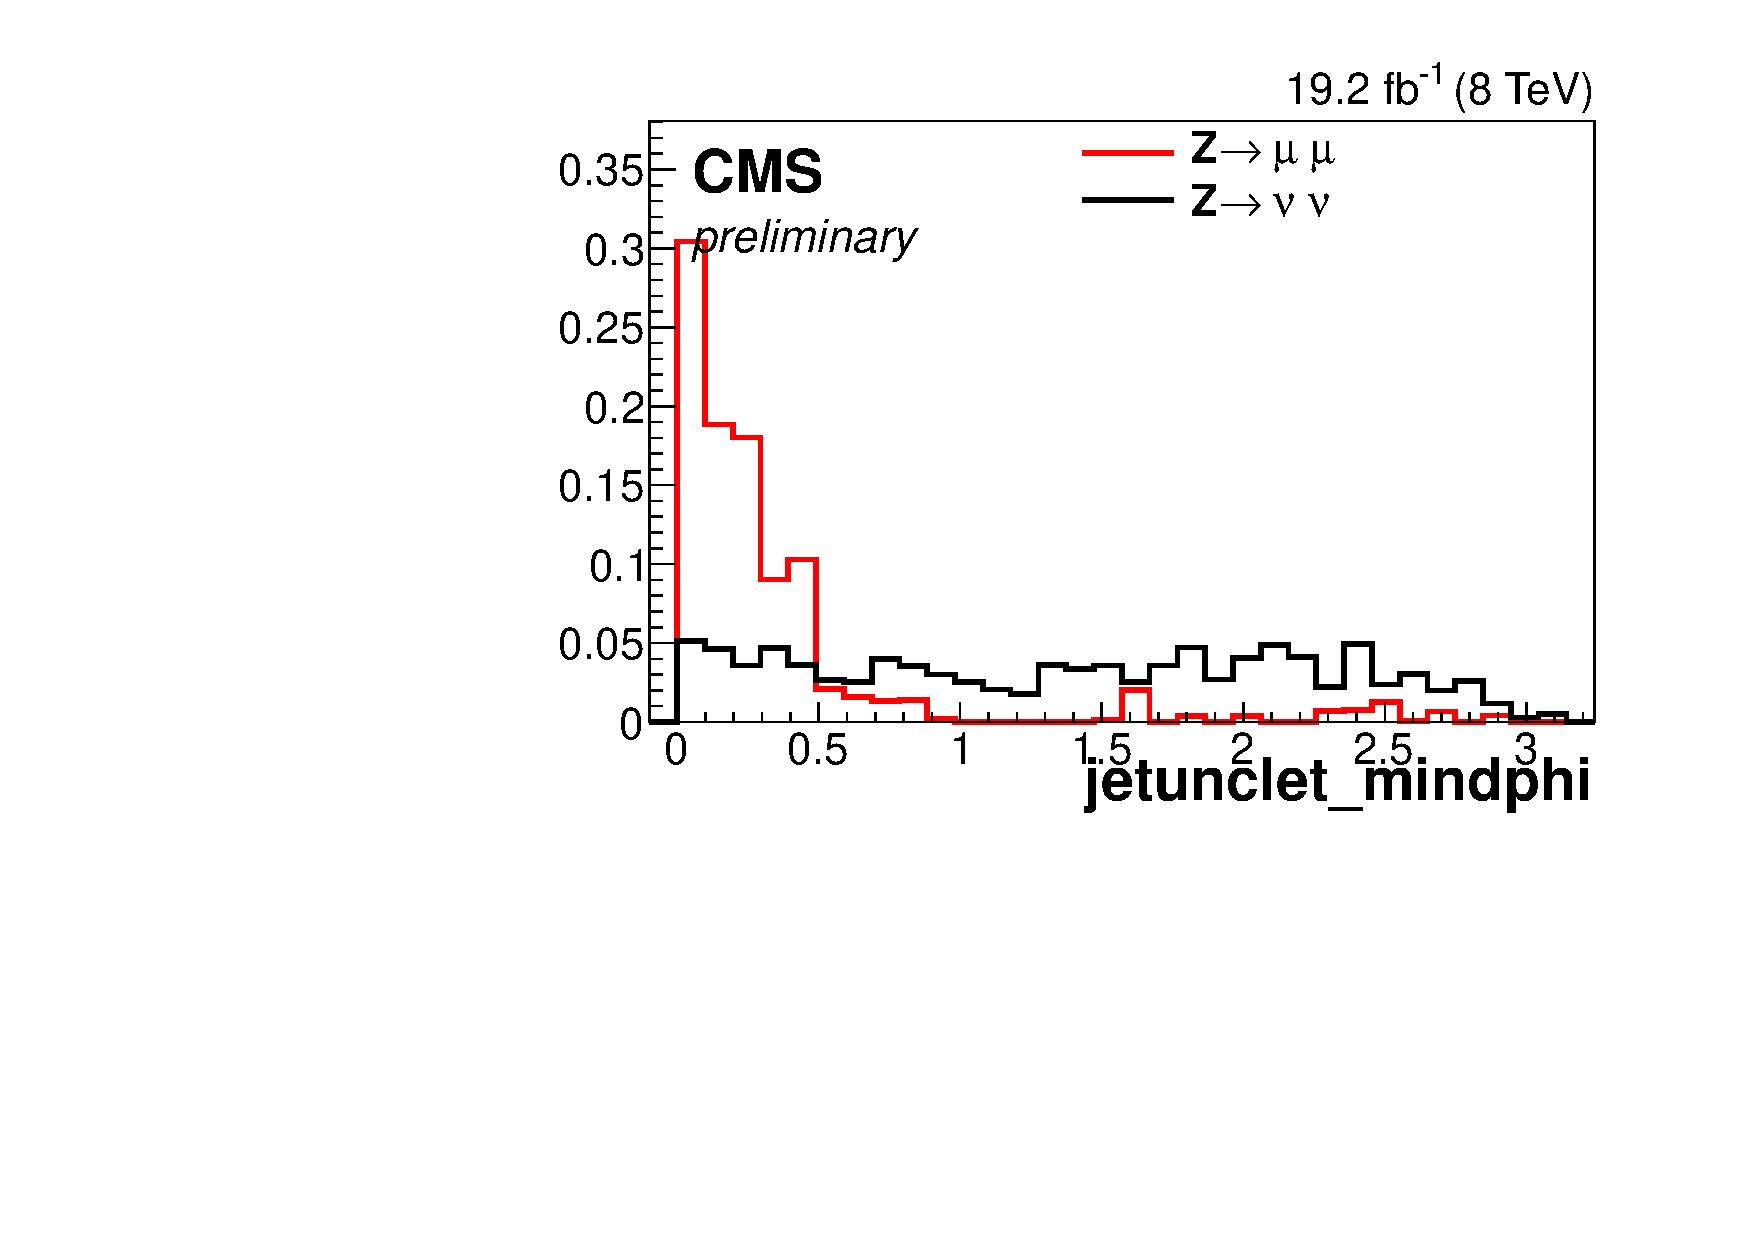
\includegraphics[width=.5\textwidth]{TalkPics/znunumcstudy200415/znunustudy_jetunclet_mindphi.pdf}
  
  \begin{block}{}
    \scriptsize
    \begin{itemize}
    \item $Z\rightarrow\mu\mu$ events always have met opposite and jets aligned with unclustered
    \end{itemize}
  \end{block}

\end{frame}

\begin{frame}
  \frametitle{Unclustered issue}
  \begin{block}{}
    \scriptsize
    \begin{itemize}
    \item Check definition of unclustered
      \begin{align*}
         \overrightarrow{\rm{Unclustered}}&=mET-mhT\\
         &= -\sum \overrightarrow{\rm{all\,pF\,candidates}} + \sum \overrightarrow{\rm{jets}}\\
         &= -\sum \overrightarrow{\rm{all\,nonjet\,pF\,candidates}}
      \end{align*}
    \item Jet collection that was used to generate unclustered has been cleaned for leptons
    \item Unclustered in events with leptons is therefore opposite the leptons
    \item This explains the behaviour seen on the previous slide
    \end{itemize}
  \end{block}
\end{frame}

\begin{frame}
  \frametitle{Summary}
  \label{lastframe}
  \begin{block}{}
    \scriptsize
    \begin{itemize}
    \item $Z\rightarrow\nu\nu$ sample looks very similar to $Z\rightarrow\mu\mu$ sample in signal region
    \item[-] Only difference is understood and not in a variable used in the analysis
    \item Therefore not likely to be cause of difference with ATLAS
    \item[-] Could study looser regions
    \item In run 2 there is a request for an EWK $Z\rightarrow\nu\nu$ sample
    \item We could maybe use these and drop the different Z background method
    \item[-] Better stats and fewer theory uncertainties
    \end{itemize}
  \end{block}
\end{frame}

\begin{frame}
  \frametitle{Backup}
\end{frame}

\end{fmffile}
\end{document}
